\documentclass[12pt]{article}
\usepackage{amsmath}
\usepackage{amssymb}
\usepackage{graphicx}
\usepackage{enumitem}
\usepackage{mathtools}
\usepackage{textcomp}
\usepackage[left=2cm,right=2cm,top=2cm,bottom=2cm]{geometry}
\usepackage{rsfso}
\usepackage{listingsutf8}
\usepackage{hyperref}
\usepackage{multicol}
\usepackage{tikz}
\usepackage{forest}
\everymath{\displaystyle}

\lstset{
    language=C,
    inputencoding=utf8,
    extendedchars=true,
    basicstyle=\ttfamily\footnotesize,
    numberstyle=\tiny\color{gray},
    stepnumber=1,
    numbersep=5pt,
    showstringspaces=false,
    breaklines=true,
    tabsize=1,
    literate=
        {ñ}{{\~n}}1
        {Ñ}{{\~N}}1
        {á}{{\'a}}1
        {é}{{\'e}}1
        {í}{{\'i}}1
        {ó}{{\'o}}1
        {ú}{{\'u}}1
        {Á}{{\'A}}1
        {É}{{\'E}}1
        {Í}{{\'Í}}1
        {Ó}{{\'Ó}}1
        {Ú}{{\'Ú}}1
}

\begin{document}

    \begin{titlepage}
        \centering
        
\includegraphics[width=0.3\textwidth]{../imgs/logo-uai-fic.png}

        \vspace{0.5cm}
        \textbf{\fontsize{12}{24} Ayudantía 8: Árboles en C}

        \vspace{0.5cm}
        \textbf{\fontsize{12}{24}\selectfont Profesores: Sebastián Sáez, Diego Ramos}

        \begin{center}
            \textbf{\fontsize{12}{24}\selectfont Ayudantes: Diego Duhalde, Benjamín Wiedmaier, Fernando Zamora}
        \end{center}
        \begin{center}
            \textbf{PREGUNTAS}
        \end{center}

        \begin{enumerate}[leftmargin=*]
            % EJERCICIO 1
            \item Defina qué es un grafo, diferenciando \emph{nodos} y \emph{aristas}. Además, explique la diferencia entre grafo dirigido y no dirigido, y dé un ejemplo de aplicación real para cada uno.

            % EJERICICIO 2
            \item Dado el siguiente grafo $G$:
            \begin{align*}
                N &= \{ A, B, C, D, E, F\} \\
                E &= \{ \{A, B\}, \{B, C\}, \{C, A\}, \{C, D\}, \{D, E\}, \{D, B\}, \{D, F\}, \{E, A\}, \{E, F\} \}
            \end{align*}
            \begin{enumerate}[label=\alph*)]
                \item Dibújelo y señale claramente
                \begin{itemize}
                    \item Un ciclo de $G$.
                    \item Un árbol de $G$.
                \end{itemize}
                \item Explique la principal diferencia entre un ciclo y un árbol.
                \item Proponga al menos una aplicación práctica en la que sea importante detectar ciclos o extraer árboles de un grafo, y justifique su elección.
            \end{enumerate}
            
            % EJERCICIO 3
            \item Compare brevemente (en tiempo y espacio) las dos principales representaciones de grafos: matriz de adyacencia y lista de adyacencia.

            % EJERCICIO 4
            \item Explique que es un árbol de expansión mínimo y mencione cuáles algoritmos existen para determinarlo.

            % EJERCICIO 5
            \item 
            \begin{enumerate}[label=\alph*)]
                \item Explique brevemente el algoritmo de Kruskal y mencione cómo asegura que el árbol generado es de expansión mínima. Además, escriba en C un código que implemente Kruskal para un grafo no dirigido.
                \item Haga lo mismo con el algoritmo de Prim.
                \item ¿Cuáles podrían ser las ventajas y desventajas de usar Kruskal versus Prim en la práctica? Considere aspectos como la estructura de datos utilizada, la eficiencia en distintos tipos de grafos y la facilidad de implementación.
            \end{enumerate}

            % EJERCICIO 6
            \item 
            \begin{enumerate}[label=\alph*)]
                \item Explique qué es el camino más corto y cómo el algoritmo de Dijkstra permite encontrarlo en un grafo con pesos no negativos. Además, escriba en C un código que implemente el algoritmo de Dijkstra para hallar la distancia mínima desde un nodo origen a todos los demás nodos.
                \item ¿Por qué no se pueden ocupar pesos negativos?
            \end{enumerate}
        \end{enumerate}
    \end{titlepage}

    \newpage
        \begin{center}
            \textbf{RESPUESTAS}
        \end{center}

        \begin{enumerate}
            % RESPUESTA 1
            \item Un grafo es una estructura matemática compuesta por un conjunto de nodos (o vértices) y un conjunto de aristas (o enlaces) que conectan pares de nodos. Los nodos representan entidades o puntos, mientras que las aristas representan las conexiones o relaciones entre ellos.

            La diferencia principal entre grafo dirigido y no dirigido es la orientación de las aristas:
            \begin{itemize}
                \item \textbf{Grafo dirigido:} Las aristas tienen una dirección, es decir, van de un nodo origen a un nodo destino. Ejemplo de aplicación: redes de flujo de tráfico, donde las calles pueden ser unidireccionales.
                \item \textbf{Grafo no dirigido:} Las aristas no tienen dirección, por lo que la relación entre los nodos es bidireccional. Ejemplo de aplicación: redes sociales, donde la amistad es mutua.
            \end{itemize}

            % RESPUESTA 2
            \item 
            \begin{enumerate}[label=\alph*)]
                \item El grafo $G$ se puede dibujar de la siguiente manera:

                \begin{center}
                    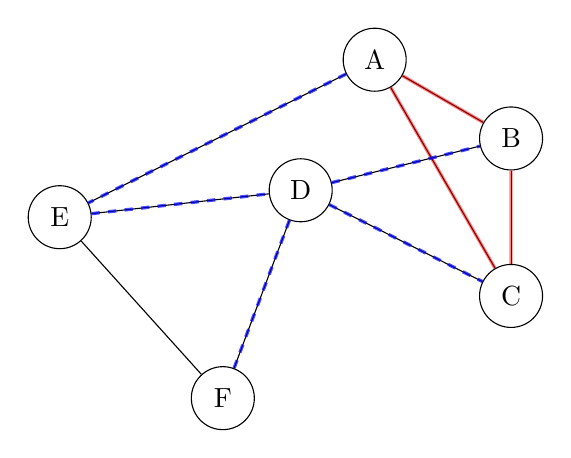
\begin{tikzpicture}[main/.style = {draw, circle, minimum size=8mm}]
                        \node[main] (A) at (90:2) {A};
                        \node[main] (B) at (30:2) {B};
                        \node[main] (C) at (330:2) {C};
                        \node[main] (D) at (160:1) {D};
                        \node[main] (E) at (180:4) {E};
                        \node[main] (F) at (230:3) {F};

                        \draw (A) -- (B);
                        \draw (B) -- (C);
                        \draw (C) -- (A);
                        \draw (C) -- (D);
                        \draw (D) -- (E);
                        \draw (D) -- (B);
                        \draw (D) -- (F);
                        \draw (E) -- (F);
                        \draw (E) -- (A);

                        \draw[red, very thick, opacity=0.5] (A) -- (B) -- (C) -- (A);
                        \draw[blue, dashed, very thick, opacity=0.7] (A) -- (E) -- (D) -- (B);
                        \draw[blue, dashed, very thick, opacity=0.7] (D) -- (C);
                        \draw[blue, dashed, very thick, opacity=0.7] (D) -- (F);
                    \end{tikzpicture}
                \end{center}
                donde, el ciclo está resaltado en \textcolor{red}{rojo} (aristas gruesas), mientras que un árbol está resaltado en \textcolor{blue}{azul} (aristas gruesas y punteadas).

                \item La principal diferencia es que un ciclo es un camino cerrado en el grafo donde se puede volver al nodo inicial sin repetir aristas ni nodos (excepto el inicial/final), mientras que un árbol es un subgrafo conexo y acíclico (no tiene ciclos).

                \item Una aplicación práctica donde es importante detectar ciclos es en la detección de dependencias circulares en sistemas de paquetes de software (para evitar bucles de dependencia). Extraer árboles es fundamental, por ejemplo, en el diseño de redes eléctricas o de comunicaciones, donde se busca conectar todos los puntos con el menor costo posible y sin ciclos (árbol de expansión mínima).
            \end{enumerate}

            % RESPUESTA 3
            \item 
            \textbf{Matriz de adyacencia:}
            \begin{itemize}
                \item \textbf{Tiempo:} Permite verificar si existe una arista entre dos nodos en tiempo $O(1)$, pero recorrer todos los vecinos de un nodo toma $O(n)$.
                \item \textbf{Espacio:} Requiere $O(n^2)$ espacio, donde $n$ es el número de nodos, ya que almacena todas las posibles conexiones.
                \item \textbf{Ventaja:} Es eficiente para grafos densos.
                \item \textbf{Desventaja:} Consume mucha memoria en grafos dispersos.
            \end{itemize}

            \textbf{Lista de adyacencia:}
            \begin{itemize}
                \item \textbf{Tiempo:} Verificar la existencia de una arista puede tomar hasta $O(\deg(v))$, donde $\deg(v)$ es el grado del nodo, y recorrer todos los vecinos también tiene complejidad $O(\deg(v))$.
                \item \textbf{Espacio:} Requiere $O(n + m)$ espacio, donde $m$ es el número de aristas, siendo mucho más eficiente para grafos dispersos.
                \item \textbf{Ventaja:} Ahorra memoria en grafos con pocas aristas.
                \item \textbf{Desventaja:} Menos eficiente para verificar la existencia de una arista específica.
            \end{itemize}

            % RESPUESTA 4
            \item Un árbol de expansión mínima (MST, por sus siglas en inglés) es un subgrafo de un grafo no dirigido, conexo y ponderado, que conecta todos los nodos con el menor peso total posible y sin formar ciclos (es decir, es un árbol). El MST contiene exactamente $n-1$ aristas si el grafo tiene $n$ nodos.

            Los algoritmos más conocidos para encontrar un árbol de expansión mínima son:
            \begin{itemize}
                \item \textbf{Kruskal:} Selecciona las aristas de menor peso y las agrega al árbol si no forman un ciclo, hasta conectar todos los nodos.
                \item \textbf{Prim:} Comienza desde un nodo y va agregando la arista de menor peso que conecta un nodo del árbol a uno fuera de él, hasta incluir todos los nodos.
            \end{itemize}

            % RESPUESTA 5
            \item 
            \begin{enumerate}[label=\alph*)]
                \item \textbf{Algoritmo de Kruskal:} Este algoritmo ordena todas las aristas del grafo por peso creciente y las va agregando al árbol de expansión si no forman un ciclo, utilizando una estructura de conjuntos disjuntos (Union-Find) para detectar ciclos. Así, siempre se agregan las aristas más baratas posibles sin cerrar ciclos, garantizando el mínimo costo total. La implementación del código la puede encontrar en la rama de ayudantías del repositorio del curso. \href{https://github.com/otrab/EDA/tree/ayudant%C3%ADas}{Link.}

                \item \textbf{Algoritmo de Prim:} Parte desde un nodo arbitrario y, en cada paso, agrega la arista de menor peso que conecta un nodo ya incluido con uno que aún no está en el árbol. Utiliza una estructura como un heap para seleccionar rápidamente la arista mínima. Lo mismo \href{https://github.com/otrab/EDA/tree/ayudant%C3%ADas}{acá}.

                \item \textbf{Ventajas y desventajas:}
                Ambos algoritmos tienen ventajas y desventajas según el tipo de grafo y la estructura de datos utilizada. Kruskal suele ser más eficiente en grafos dispersos y cuando las aristas se presentan como lista, además de ser sencillo de implementar con la estructura Union-Find; sin embargo, requiere ordenar todas las aristas, lo que puede ser costoso en grafos muy densos. Por otro lado, Prim es más eficiente en grafos densos y cuando se utiliza una matriz de adyacencia, especialmente si se emplea un heap para seleccionar la arista mínima; no obstante, puede ser menos eficiente en grafos dispersos si no se elige la estructura adecuada.
            \end{enumerate}

            % RESPUESTA 6
            \item 
            \begin{enumerate}[label=\alph*)]
                \item El \textbf{camino más corto} entre dos nodos en un grafo es la secuencia de aristas que conecta ambos nodos con el menor peso total posible. El \textbf{algoritmo de Dijkstra} permite encontrar el camino más corto desde un nodo origen a todos los demás en un grafo con pesos no negativos, utilizando una estructura de prioridad (como un heap) para seleccionar el nodo con la distancia mínima conocida en cada paso y actualizando las distancias a sus vecinos. El código lo puede encontrar \href{https://github.com/otrab/EDA/tree/ayudant%C3%ADas}{acá}.

                \item Dijkstra no funciona correctamente con pesos negativos porque podría pasar por un nodo y luego encontrar un camino más corto a ese nodo usando una arista negativa, pero el algoritmo ya habría marcado ese nodo como visitado y no actualizaría su distancia, produciendo resultados incorrectos.
            \end{enumerate}
        \end{enumerate}
\end{document}